\documentclass[a4paper,10pt]{article}

\usepackage[utf8]{inputenc} % pour les accents
\usepackage[T1]{fontenc} % caracteres francais
\usepackage{geometry} %les marges
\usepackage[french]{babel} %langue principale
\usepackage[dvips]{graphicx}
\geometry{ hmargin=2cm, vmargin=2cm }
\usepackage{lscape}
\usepackage{amsmath}
\usepackage{hyperref}

%%%%%%%%%%%%%%%%%%%%%%%%%%%%%%%%%%%%%%%%%%%%%%%%%%%%%%%%%%%%%%%%%%%%%%%%%%%%%%%%%%%%%%
%%%%%%%%%%%%%%%%%%%%%%%%%%%%%%%%%% DEBUT DU DOCUMENT %%%%%%%%%%%%%%%%%%%%%%%%%%%%%%%%%
%%%%%%%%%%%%%%%%%%%%%%%%%%%%%%%%%%%%%%%%%%%%%%%%%%%%%%%%%%%%%%%%%%%%%%%%%%%%%%%%%%%%%%

\begin{document}

\begin{titlepage}
\begin{center}

% Author and supervisor
\begin{minipage}{0.4\textwidth}
\begin{flushleft} \large

\includegraphics[scale=0.4]{./EDF_Logo}
\end{flushleft}
\end{minipage}
\begin{minipage}{0.4\textwidth}
\begin{flushright} \large
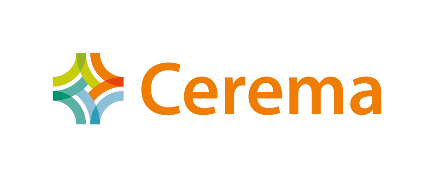
\includegraphics[scale=1.]{./CEREMA_Logo}
\end{flushright}
\end{minipage}

% Upper part of the page
\textsc{ }\\[7cm]
\textsc{\Huge MASCARET v8.1}\\[1cm]
{ \huge \bfseries Module de calcul de capacit\'e de transport de s\'ediments MASCAPA}\\[1cm]
\textsc{\Large NOTE DE PRINCIPE}\\
\vfill

% Bottom of the page
{\Large Copyright {\copyright} 2015 EDF - CEREMA}\\[0.5cm]
{EDF - SA au capital de 924.433.331 euros - R.C.S. Paris B 552 081 317}\\
{CEREMA - Centre d'\'etudes et d'expertise sur les risques, l'environnement, la mobilit\'e et l'am\'enagement}

\end{center}
\end{titlepage}

%%%%%%%%%%%%%%%%%%%%%%%%%%%%%%%%%%%%%%%%%%%%%%%%%%%%%%%%%%%%%%%%%%%%%%%%%%%%%%%%%%%%%
%%%%%%%%%%%%%%%%%%%%%%%%%%%%%%%%%%%%%%% RÉSUMÉ %%%%%%%%%%%%%%%%%%%%%%%%%%%%%%%%%%%%%%
%%%%%%%%%%%%%%%%%%%%%%%%%%%%%%%%%%%%%%%%%%%%%%%%%%%%%%%%%%%%%%%%%%%%%%%%%%%%%%%%%%%%%

\newpage
\titlepage{
\begin{LARGE}
\begin{center}
R\'esum\'e
 \end{center}
 \end{LARGE}}

\noindent
Fudaa-Mascapa est le module de calcul de capacit\'e de transport de l'outil num\'erique MASCARET \cite{gou1}, code de calcul d'hydraulique \`a surface libre monodimensionnel. Il calcule le d\'ebit solide par charriage ou transport total dans une rivi\`ere. \\

\noindent
Le d\'ebit solide annuel en chaque section du cours d'eau peut \^etre d\'eduit, et des bilans s\'edimentaires par tron\c con peuvent \^etre calcul\'es. \\

\noindent
A noter que la structure du module, cod\'e en Java, permet une \'evolution ais\'ee vers des fonctionnalit\'es plus complexes : prise en compte d'affluents, de singularit\'es, voire de la gestion des fonds. \\

\noindent
Ce rapport est la note de principe du code.

%%%%%%%%%%%%%%%%%%%%%%%%%%%%%%%%%%%%%%%%%%%%%%%%%%%%%%%%%%%%%%%%%%%%%%%%%%%%%%%%%%%%%
%%%%%%%%%%%%%%%%%%%%%%%%%%%%%%%%% TABLE DES MATIÈRES %%%%%%%%%%%%%%%%%%%%%%%%%%%%%%%%
%%%%%%%%%%%%%%%%%%%%%%%%%%%%%%%%%%%%%%%%%%%%%%%%%%%%%%%%%%%%%%%%%%%%%%%%%%%%%%%%%%%%%

\newpage
\begin{center} Sommaire/Summary
\end{center}\
\tableofcontents

%%%%%%%%%%%%%%%%%%%%%%%%%%%%%%%%%%%%%%%%%%%%%%%%%%%%%%%%%%%%%%%%%%%%%%%%%%%%%%%%%%%%%
%%%%%%%%%%%%%%%%%%%%%%%%%%%%%%%%%%%%%% NOTATION %%%%%%%%%%%%%%%%%%%%%%%%%%%%%%%%%%%%%
%%%%%%%%%%%%%%%%%%%%%%%%%%%%%%%%%%%%%%%%%%%%%%%%%%%%%%%%%%%%%%%%%%%%%%%%%%%%%%%%%%%%%

\newpage
\titlepage{
\begin{LARGE}
\begin{center}
Notations
\end{center}
\end{LARGE}}
\begin{tabular}{ l l }

\textbf{Notation}		& $ $ \\ [0.2 cm]
$D_i$					& Diam\`etre majorant des diam\`etre de i\% de la masse solide \\
$D_{50}$				& Diam\`etre m\'edian \\
$D_m$					& Diam\`etre moyen arithm\'etique $ = \sum d_i p_i $ \\
$ $						& ($p_i$ est le pourcentage en masse de particules de diam\`etre $d_i$) \\
$D^*$					& Diam\`etre adimensionnel = $D_m \left[\frac{g(s-1)}{\nu^2}\right]^{1/3}$ \\
$F_r$					& Nombre de Froude ($ F_r = \frac{U}{ \sqrt{gH} } $) \\
$H$						& Profondeur de l'\'ecoulement \\
$K$						& Coefficient de Strickler de l'\'ecoulement \\
$K_r$					& Coefficient de Strickler pour les grains $ (K_r = \frac{21.1}{D_m^{1/6}}) $ ou \\
$ $						& $ (K_r = \frac{26}{D_{90}	^{1/6}}) $ pour la formule de Meyer-Peter \& M\"uller \\
$L$						& Largeur du lit \\
$Q$						& D\'ebit \\
$q$						& D\'ebit unitaire ($q = Q/L$) \\
$Q_s$					& D\'ebit solide (ou capacit\'e de transport solide) en $kg/s$ \\
$q_s$					& D\'ebit solide unitaire ($q_s = Q_s / L$) \\
$R_h$					& Rayon hydraulique \\
$Re$					& Nombre de Reynolds ($Re = UH / \nu$) \\
$Re^*$					& Nombre de Reynolds particulaire ($Re^* = u^* D / \nu$) \\
$S$						& Pente d'\'energie ou de fond \\
$s$						& Densit\'e relative ($s = \rho_s/\rho$) \\
$T$						& Param\`etre adimensionnel de transport solide $ = \frac{u^{*2}-u_c^{*2}}{u_c^{*2}} $ \cite{van1}\\
$U$						& Vitesse moyenne \\
$u^*$					& Vitesse de frottement $ = \sqrt{\tau/\rho} = \sqrt{gHS} $ \\ [0.1 cm]
$u^*_c$					& Vitesse de frottement critique $ = \sqrt{\tau_c/\rho} $ \\
$\alpha$				& Angle de frottement interne de s\'ediment \\
$\nu$					& Viscosit\'e cin\'ematique de l'eau \\
$\Phi$					& Transport solide adimensionnel $ = \frac{ {14\theta}^{2.5} }{ [1 + (\theta_m/\theta)^4] } $ \\ 
$\rho$					& Masse volumique d'eau \\
$\rho_s$				& Masse volumique des s\'ediments \\
$\tau$					& Contrainte moyenne au fond \\
$\tau_{e}$				& Contrainte efficace \\
$\theta_m$				& Seuil de mobilit\'e pour la fraction grossi\`ere uniquement ($D_{84}$ dans la formule de Recking 2011) \\
$\theta$				& Nombre de Shields \\
$\theta_c$				& Nombre de Shields critique pour le d\'ebut du mouvement \\


\end{tabular}
\\ [0.5 cm]

\noindent
Sauf indication contraire, le rayon hydraulique est $ R_h = (H \times L)/(L+2H) $, sous l'hypoth\`ese d'une section d'\'ecoulement rectangulaire. Cette hypoth\`ese est r\'ealis\'ee pour homog\'en\'eiser les r\'esultats: certaines formules ayant int\'egr\'e cette hypoth\'ese de fa\c con explicite, d'autres de fa\c con moins explicite. \\

%%%%%%%%%%%%%%%%%%%%%%%%%%%%%%%%%%%%%%%%%%%%%%%%%%%%%%%%%%%%%%%%%%%%%%%%%%%%%%%%%%%%%
%%%%%%%%%%%%%%%%%%%%%%%%%%%%%%%%% OBJECTIFS DU CODE %%%%%%%%%%%%%%%%%%%%%%%%%%%%%%%%%
%%%%%%%%%%%%%%%%%%%%%%%%%%%%%%%%%%%%%%%%%%%%%%%%%%%%%%%%%%%%%%%%%%%%%%%%%%%%%%%%%%%%%

\newpage
\section{Objectifs du Code}

\noindent
L'\'evolution des rivi\`eres \`a grandes \'echelles de temps et d'espace fait maintenant partie des pr\'eoccupations environnementales. Les d\'eveloppements humains et l'extraction des mat\'eriaux dans les rivi\`eres m\`enent \`a la transformation des cours d'eaux naturels. La volont\'e de limiter l'impact de l'\'evolution morphologique des rivi\`eres am\'enag\'ees sur l'environnement ou m\^eme sur les activit\'es humaines pose le probl\`eme de la repr\'esentation de ces \'evolutions sur le long terme. \\

\noindent
Il y a donc un besoin d'une meilleure compr\'ehension de processus hydros\'edimentaires qui conditionnent l'\'evolution morphologique des cours d'eau. \\

\noindent
La mod\'elisation \`a grande \'echelle de la dynamique hydros\'edimentaire peut servir d'appui \`a la d\'efinition d'un plan de gestion durable et rationel du syst\`eme fluvial, ainsi que pr\'evoir si besoin des travaux de restauration \'ecologique. L'un des objectifs du module Fudaa-Mascapa, int\'egr\'e dans le logiciel MASCARET du LNHE, EDF, R\&D, est ainsi de pr\'edire l'evolution d'un cours d'eau sur le long terme (ann\'ee apr\`es ann\'ee) au travers d'une approche simplifi\'ee bas\'ee sur les bilans s\'edimentaires. \\

\noindent
Fudaa-Mascapa est capable de calculer, en chaque section du cours d'eau, les taux annuels de transport solide selon diff\'erentes formules empiriques. Des bilans s\'edimentaires par tron\c con peuvent \^etre d\'eduits afin d'appr\'ehender les tendances d'\'evolution du lit. \\

\noindent
La structure du module, cod\'e en Java, permet une \'evolution ais\'ee vers des fonctionnalit\'es plus complexes : prise en compte d'affluents, de singularit\'es voire de la deformation des fonds. \\

\noindent
Ce document constitue la note de principe de Fudaa-Mascapa.

%%%%%%%%%%%%%%%%%%%%%%%%%%%%%%%%%%%%%%%%%%%%%%%%%%%%%%%%%%%%%%%%%%%%%%%%%%%%%%%%%%%%%
%%%%%%%%%%%%%%%%%%%%%%%%%%%%%%%%% PRINCIPE PHYSIQUE %%%%%%%%%%%%%%%%%%%%%%%%%%%%%%%%%
%%%%%%%%%%%%%%%%%%%%%%%%%%%%%%%%%%%%%%%%%%%%%%%%%%%%%%%%%%%%%%%%%%%%%%%%%%%%%%%%%%%%%

\section{Principes Physiques}

%%%%%%%%%%%%%%%%%%%%%%%%%%%%%%%%%%%%%%%%%%%%%%%%%%%%%%%%%%%%%%%%%%%%%%%%%%%%%%%%%%%%%
%%%%%%%%%%%%%%%%%%%%%%%%%%%%%%%% HYPOTHÈSES GÉNÉRALES %%%%%%%%%%%%%%%%%%%%%%%%%%%%%%%
%%%%%%%%%%%%%%%%%%%%%%%%%%%%%%%%%%%%%%%%%%%%%%%%%%%%%%%%%%%%%%%%%%%%%%%%%%%%%%%%%%%%%

\subsection{Hypoth\`eses g\'en\'erales}

\noindent
Le module calcule la capacit\'e de transport solide d'un \'ecoulement le long d'un bief. Le bief est mod\'elis\'e selon les hypoth\`eses du code de calcul MASCARET. La g\'eom\'etrie est d\'ecrite par des profils en travers, entre lesquels des sections de calcul sont interpol\'ees. L'utilisation de MASCARET permet d'obtenir au droit de chaque section la surface mouill\'ee, la vitesse, le p\'erim\`etre mouill\'e et le tirant d'eau pour chacun des d\'ebits simul\'es.  \\

\noindent
Les r\'esultats des calculs hydrauliques r\'ealis\'es par MASCARET sur le bief sont des donn\'ees d'entr\'ee de MASCAPA. On suppose donc que les variables hydrauliques sont connues de m\^eme que la rugosit\'e totale du lit (exprim\'ee par le coefficient de Strickler dans MASCARET). Ceux-ci ne sont pas modifi\'es par le transport solide pendant la simulation. \\

\noindent
Les unit\'es du transport solide donn\'e par chacune des formulation impl\'ement\'ees sont en $m^3/s$. Cependant MASCAPA fournit le d\'ebit solide en $kg/s$. Pour cela il multiplie le d\'ebit solide volum\'etrique par $\rho_s$. \\

\noindent
Diff\'erentes formules issues de la litt\'erature sont impl\'ement\'ees dans Fudaa-Mascapa. Elles s'appuient sur la notion d'une contrainte ou d'un d\'ebit seuil, responsable du d\'ebut de transport solide. La contrainte hydraulique s'exprime par :
$$ \tau_h = \rho g R_h S $$ 

La contrainte adimensionelle (ou nombre de Shields) est donn\'ee par la relation :
$$ \theta = \frac{\tau}{\rho g (s-1) D} = \frac{R_h S}{(s-1) D} $$

o\`u $D$ est \'egal \`a $D_{50}$ ou $D_m$ selon les formules. \\

La contrainte efficace est li\'ee \`a la rugosit\'e de grain, selon la relation suivante :
$$ \tau_{e} = \tau_h \cdot \left(\frac{K}{K_r}\right)^{3/2} $$

%%%%%%%%%%%%%%%%%%%%%%%%%%%%%%%%%%%%%%%%%%%%%%%%%%%%%%%%%%%%%%%%%%%%%%%%%%%%%%%%%%%%%%
%%%%%%%%%%%%%%%%%%%%%%%%%%%% DÉBIT SOLIDE LE LUNG DU BIEF %%%%%%%%%%%%%%%%%%%%%%%%%%%%
%%%%%%%%%%%%%%%%%%%%%%%%%%%%%%%%%%%%%%%%%%%%%%%%%%%%%%%%%%%%%%%%%%%%%%%%%%%%%%%%%%%%%%

\subsection{D\'ebit solide le long du bief}

\noindent
Le logiciel se limite au transport de s\'ediments granulaires par charriage ou total (charriage et suspension). \\

\noindent
Les formules prises en compte sont les suivantes :
\begin{itemize}
\item Formule de Meyer-Peter \& M\"uller (1948)
\item Formule d'Engelund \& Hansen (1967)
\item Formule de Smart \& J\"aggi (1983)
\item Formule de Van Rijn (1984)
\item Formule de Rieckenmann (1990)
\item Formules de Lefort (1991 et 2007)
\item Formules de Recking (2010 et 2011) \\
\end{itemize}

%%%%%%%%%%%%%%%%%%%%%%%%%%%%%%%%%%%%%%%%%%%%%%%%%%%%%%%%%%%%%%%%%%%%%%%%%%%%%%%%%%%%%%
%%%%%%%%%%%%%%%%%%%%%%%%%%%%%% MEYER-PETER MÜLLER 1948 %%%%%%%%%%%%%%%%%%%%%%%%%%%%%%%
%%%%%%%%%%%%%%%%%%%%%%%%%%%%%%%%%%%%%%%%%%%%%%%%%%%%%%%%%%%%%%%%%%%%%%%%%%%%%%%%%%%%%%

\subsubsection{Formule de Meyer-Peter \& M\"uller (1948)}

\noindent
La formule de Meyer-Peter \& M\"uller (1948) est issue d'exp\'eriences en laboratoires. Elle est adapt\'ee aux cas de transport par charriage soit pour des contraintes hydrodynamiques adimensionelles $\theta$ inf\'erieures \`a 0.3. Elle a \'et\'e cal\'ee pour des diam\`etres s'\'etendant de 0.4 \`a 29 mm et des pentes de fond de 0.4 \`a 2.4 \%. La formule utilise le diam\`etre $D_m$. \\

\noindent
Elle fait intervenir les deux param\`etres suivants :
\begin{itemize}
\item la contrainte adimensionelle de d\'ebut d'entra\^inement $\theta_c$, qui est \'egale \`a 0.047, et
\item la contrainte efficace $\theta_{eff}$ qui est donn\'ee par : $\left(\frac{K}{K_r}\right)^{3/2} \theta $ avec $K_r = \frac{26}{D_{90}^{1/6}}$
\end{itemize}

\noindent
Si $\theta_{eff} < \theta_c$, le d\'ebit solide $Q_s$ (en $m^3/s$) est \'egal \`a 0.

\noindent
Sinon il est donn\'e par la formule suivante :
$$ Q_s = 8 L \sqrt{g (s-1) D_m^3} (\theta_{eff} - \theta_c)^{3/2} $$

%%%%%%%%%%%%%%%%%%%%%%%%%%%%%%%%%%%%%%%%%%%%%%%%%%%%%%%%%%%%%%%%%%%%%%%%%%%%%%%%%%%%%%%
%%%%%%%%%%%%%%%%%%%%%%%%%%%%%%%%% ENGLUND HANSEN 1967 %%%%%%%%%%%%%%%%%%%%%%%%%%%%%%%%%
%%%%%%%%%%%%%%%%%%%%%%%%%%%%%%%%%%%%%%%%%%%%%%%%%%%%%%%%%%%%%%%%%%%%%%%%%%%%%%%%%%%%%%%

\subsubsection{Formule d'Engelund \& Hansen (1967)}

\noindent
La formule d'Engelund \& Hansen (1967) s'appuie sur des exp\'eriences en laboratoire. Elle s'applique \`a des grains de diam\`etre compris entre 0.15 et 1.6 mm et pour des pentes de fond faibles. La formule utilise le diam\`etre $D_{50}$ et donne le d\'ebit solide total (en $m^3/s$) sous la forme :

$$ Q_s = L \frac{0.1}{f} \sqrt{g (s-1) D_{50}^3} \theta^{5/2} $$

avec :

$$ f = \frac{2 g R_h S}{U^2} $$

%%%%%%%%%%%%%%%%%%%%%%%%%%%%%%%%%%%%%%%%%%%%%%%%%%%%%%%%%%%%%%%%%%%%%%%%%%%%%%%%%%%%%%
%%%%%%%%%%%%%%%%%%%%%%%%%%%%%%%%%% SMART JÄGGI 1983 %%%%%%%%%%%%%%%%%%%%%%%%%%%%%%%%%%
%%%%%%%%%%%%%%%%%%%%%%%%%%%%%%%%%%%%%%%%%%%%%%%%%%%%%%%%%%%%%%%%%%%%%%%%%%%%%%%%%%%%%%


\subsubsection{Formule de Smart \& J\"aggi (1983)}

\noindent
La formule de Smart \& J\"aggi (1983) s'appuie sur des exp\'eriences en laboratoire \cite{sma1}. Elle s'applique \`a des grains de diam\`etre compris entre 2 et 10.5 mm et pour des pentes de fond comprises entre 3 et 20 \%. La formule utilise les trois diam\`etres $D_{m}$, $D_{90}$ et $D_{30}$. \\

\noindent
Le d\'ebit solide $Q_s$ (en $m^3/s$) est donn\'e par la formule suivante :
$$ Q_s = 4 Q \left(\frac{D_{90}}{D_{30}}\right)^{0.2} \frac{S^{1.6}}{(s-1)} \left(1-\frac{\theta_c}{\theta}\right) $$

o\`u la contrainte critique adimensionnel $\theta_c$ est donn\'ee par :
$$ \theta_c = 0.05 \cos( \arctan(S) ) \left(1-\frac{S}{\tan \varphi}\right) $$

\indent
avec $\varphi = 35\,^{\circ}$ = angle de frottement interne du mat\'eriau.

%%%%%%%%%%%%%%%%%%%%%%%%%%%%%%%%%%%%%%%%%%%%%%%%%%%%%%%%%%%%%%%%%%%%%%%%%%%%%%%%%%%%%%%
%%%%%%%%%%%%%%%%%%%%%%%%%%%%%%%%%%%% VAN RIJN 1984 %%%%%%%%%%%%%%%%%%%%%%%%%%%%%%%%%%%%
%%%%%%%%%%%%%%%%%%%%%%%%%%%%%%%%%%%%%%%%%%%%%%%%%%%%%%%%%%%%%%%%%%%%%%%%%%%%%%%%%%%%%%%

\subsubsection{Formule de Van Rijn (1984)}

\noindent
La formule de Van Rijn (1984) est une m\'ethode semi-empirique valid\'ee pour les sables \cite{van1}. Elle s'applique \`a des grains de diam\`etre compris entre 0.2 et 2 mm. La formule utilise les deux diam\`etres $D_{50} $ et $ D_{90}$. \\

\noindent
Le d\'ebit solide $Q_s$ (en $m^3/s$) est donn\'e sous la forme :
$$ Q_s = 0.053 L \sqrt{g (s-1) D_{50}^3} \frac{T^{2.1}}{D_*^{0.3}} $$

\noindent
et fait intervenir les param\`etres suivants :
\begin{itemize}
\item le param\`etre $T$
$$ T = \frac{u^{*2}-u_c^{*2}}{u_c^{*2}} $$

\item le param\`etre $u^*$
$$ u^* = \sqrt{g} \frac{U}{18 \log\left(\frac{4R_h}{D_{90}}\right) } $$

\item le param\`etre $u_c^{*2}$, calcul\'e via la courbe de Shields donn\'ee par la forme suivante :
$$ u_c^{*2} = g (s-1) \cdot D_{50} \cdot [ \alpha \cdot D_*^\beta ] = g (s-1) \cdot D_{50} \cdot \theta $$

avec

$$ D_* = D_{50} \left[\frac{g(s-1)}{\nu^2}\right]^{1/3} $$

\begin{center}
\begin{tabular}{| c | c | c |}
\hline
$D_*$			& $\alpha$		& $\beta$	\\ \hline
$D_* < 4$		&	0.24		& -1		\\
$4<D_*<10$		&	0.14		& -0.64		\\
$10<D_*<20$		&	0.04		& 0.1		\\
$20<D_*<150$	&	0.013		& 0.29		\\
$150<D_*$		&	0.055		& 0			\\ \hline
\end{tabular}
\end{center}
\end{itemize}


%%%%%%%%%%%%%%%%%%%%%%%%%%%%%%%%%%%%%%%%%%%%%%%%%%%%%%%%%%%%%%%%%%%%%%%%%%%%%%%%%%%%%%
%%%%%%%%%%%%%%%%%%%%%%%%%%%%%%%%%% RIECKENMANN 1990 %%%%%%%%%%%%%%%%%%%%%%%%%%%%%%%%%%
%%%%%%%%%%%%%%%%%%%%%%%%%%%%%%%%%%%%%%%%%%%%%%%%%%%%%%%%%%%%%%%%%%%%%%%%%%%%%%%%%%%%%%

\subsubsection{Formule de Rieckenmann (1990)}

\noindent
La formule de Rieckenmann (1990) s'appuie sur des exp\'eriences en laboratoire. Elle s'applique \`a des grains de diam\`etre compris entre 0.4 et 10 mm et pour des pentes de fond comprises entre 0.0004 et 0.2 \%. La formule utilise les trois diam\`etres  $D_{50}$, $D_{90}$ et $D_{30}$. \\

\noindent
Le d\'ebit solide $Q_s$ (en $m^3/s$) pour les pentes de fond $S < 0.03 \%$ est sous la forme :
$$ Q_s = 1.5 L (q - q_c) S^{1.5} $$

\noindent
Pour $S > 0.03 \%$, $Q_s$ prend la forme :
$$ Q_s = L \frac{12.6}{(s-1)^{1.6}} \left(\frac{D_{90}}{D_{30}}\right)^{0.2} (q - q_c) S^2$$ 

\noindent
avec le d\'ebit de d\'ebut d'entra\^inement $Q_c$ (en $m^3/s$) :
$$ Q_c = 0.065 (s-1)^{5/3} g^{0.5} D_{50}^{1.5} S^{-1.12} $$

%%%%%%%%%%%%%%%%%%%%%%%%%%%%%%%%%%%%%%%%%%%%%%%%%%%%%%%%%%%%%%%%%%%%%%%%%%%%%%%%%%%%%%
%%%%%%%%%%%%%%%%%%%%%%%%%%%%%%%%%%%% LEFORT 1991 %%%%%%%%%%%%%%%%%%%%%%%%%%%%%%%%%%%%%
%%%%%%%%%%%%%%%%%%%%%%%%%%%%%%%%%%%%%%%%%%%%%%%%%%%%%%%%%%%%%%%%%%%%%%%%%%%%%%%%%%%%%%

\subsubsection{Formule de Lefort (1991)}

\noindent
La formule de Lefort (1991) donne le d\'ebit solide sans faire intervenir la largeur de la rivi\`ere.\\

\noindent
L'utilisation de la formule Lefort (1991), formule cal\'ee sur les essais de laboratoire de Meyer-Peter \& M\"uller et plus tard de Smart \& J\"aggi, se limite \`a des pentes de 0.25 \`a 2.4 \%. La formule utilise les trois diam\`etres $D_m$, $D_{90}$ et $D_{30}$. Elle donne le d\'ebit solide apparent (tenant compte des vides) et consid\`ere un ratio largeur-hauteur du lit $L/h = 18$. \\*

\noindent
La formule originale de Lefort est (en $m^3/s$) :
$$ Q_{s, app} = 4.45 Q \left(\frac{D_{90}}{D_{30}}^{0.2}\right) \frac{S^{1.5}}{(s-1)} \left[1 - \left(\frac{Q_c}{Q}\right)^{0.375}\right] $$

\noindent
Le d\'ebit solide est reli\'e au d\'ebit solide apparent par $ Q_s =  0.755 \cdot Q_{s, app}$ (calcul\'e en prenant la densit\'e apparente \'egale \`a 2 et une densit\'e des mat\'eriaux \'egale \`a 2.65), soit:

$$ Q_s = 3.36 Q \left(\frac{D_{90}}{D_{30}}^{0.2}\right) \frac{S^{1.5}}{(s-1)} \left[1 - \left(\frac{Q_c}{Q}\right)^{0.375}\right] $$ \\

\noindent
avec le d\'ebit de d\'ebut d'entra\^inement $Q_c$ (en $m^3/s$) :
$$ Q_c = 0.0776 \sqrt{g D_m^5} \frac{(s-1)^{8/3}}{S^{13.6}} (1-1.2 S)^{8/3} $$

%%%%%%%%%%%%%%%%%%%%%%%%%%%%%%%%%%%%%%%%%%%%%%%%%%%%%%%%%%%%%%%%%%%%%%%%%%%%%%%%%%%%%%
%%%%%%%%%%%%%%%%%%%%%%%%%%%%%%%%%%%% LEFORT 2007 %%%%%%%%%%%%%%%%%%%%%%%%%%%%%%%%%%%%%
%%%%%%%%%%%%%%%%%%%%%%%%%%%%%%%%%%%%%%%%%%%%%%%%%%%%%%%%%%%%%%%%%%%%%%%%%%%%%%%%%%%%%%

\subsubsection{Formule de Lefort (2007)}

\noindent
La formule Lefort (2007) s'appuie sur des exp\'eriences en laboratoire. Elle s'applique \`a des grains de diam\`etre compris entre 0.1 et 55 mm et pour des pentes de fond allant jusqu'\`a 20 \%. La formule utilise les diam\`etres $D_m$, $D_{90}$ et $D_{30}$. Le d\'ebit solide calcul\'e inclut le charriage et la suspension.\\ 

\noindent
Le d\'ebit solide $Q_s$ (en $m^3/s$) est donn\'e par :
$$Q_s = \frac{C_p \cdot Q}{s \cdot 10^6} $$

\noindent
o\`u la concentration $C_p$ \cite{lef1} est \'egale \`a : 
$$C_p = 3.176 \cdot 10^6 \cdot cor \cdot \left(\frac{D_{90}}{D_{30}}\right)^{0.21} \frac{s}{(s-1)^{1.38}} S^m [G(Q^*)]^Z$$

\noindent
La concentration $C_p$ fait intervenir les param\`etres $cor$, $m$, $G(Q^*)$, et $Z$ : \\

\begin{itemize}
\item $cor$ est un coefficient de correction qui tient compte de l'effet des dunes. \\

$cor = 1 - 9 e^{(-0.08 \cdot Q^* \left(\frac{K}{Kr}\right)^{2.4})}$ si $\frac{K}{Kr} < 0.6$; sinon $cor = 1$ \\

\item l'exposant $m$ : $ m = 1.887 + 0.09 \log(S) $ \\

\item le calcul de la fonction $G(Q^*)$ n\'ecessite le calcul du debit de mise en mouvement $Q_c$ (en $m^3/s$), donn\'e sous la forme suivante :

$$ Q_c = \sqrt{g D_m^5} C_{(D_m^*)} (s-1)^{5/3} \left(\frac{L}{D_m}\right)^{2/3} \left(\frac{K}{Kr}\right)^{-0.42} S^{-n} $$

avec $n = 1.725 + 0.09 \log(S)$ \\

$C_{(D_m^*)}$ est donn\'e par : \\

\begin{center}
$C_{(D_m^*)} = 0.0269$ si $D_m < 0.008$ \\
sinon $C_{(D_m^*)} = 0.0269 + \frac{0.532}{(1.1 + D_m^*)} - 0.0589 \exp^{-D_m^*/60}$ \\ [0.2 cm]
\end{center}

Finalement $G(Q^*)$ est donn\'e par :

$ G(Q^*) = 3.88 \left[ 1 - \left(\frac{0.75}{Q^*}\right)^{0.25} \right]^{5/3} $ si $ Q^* > 2.5 $

$ G(Q^*) = 0.4 \left[\frac{Q^*}{2.5}\right]^{6.25(1-0.37Q^*)} $ si $ Q^* < 2.5 $\\

avec $Q^* = \frac{Q}{Q_c}$ \\

\item l'exposant $Z$ est donn\'e sous la forme :

$$ Z = 0.78 + \frac { 1.53 Re^{0.14} }{ {D_m^*}^{0.78} } $$

avec

$$ Rh = \frac{h L}{L+2h}; Re = \frac{Q R_h}{L h \nu} $$
\end{itemize}

%%%%%%%%%%%%%%%%%%%%%%%%%%%%%%%%%%%%%%%%%%%%%%%%%%%%%%%%%%%%%%%%%%%%%%%%%%%%%%%%%%%%%%
%%%%%%%%%%%%%%%%%%%%%%%%%%%%%%%%%%%% RECKING 2010 %%%%%%%%%%%%%%%%%%%%%%%%%%%%%%%%%%%%
%%%%%%%%%%%%%%%%%%%%%%%%%%%%%%%%%%%%%%%%%%%%%%%%%%%%%%%%%%%%%%%%%%%%%%%%%%%%%%%%%%%%%%

\subsubsection{Formule de Recking (2010)}

\noindent
La formule de Recking (2010) s'appuie sur des exp\'eriences en laboratoire et des mesures en terrain. Elle s'applique \`a des grains de diam\`etre compris entre 0.4 et 220 mm et pour des pentes de fond comprises entre 0.001 et 7 \%. La formule utilise les deux diam\`etres $D_{50}$ et $D_{84}$. \\

\noindent
Dans cette formule, le diam\`etre $D$ est d\'efini par $3.5 D_{84}$ pour les rivi\`eres \`a graviers ($ D_{50} > 0.002 mm$) et par $D_{50} $ pour les rivi\`eres \`a sable. \\

\noindent
Le rayon hydraulique $R_{hg}$ (utilis\'e pour le calcul de $\theta$) est donn\'e par l'\'equation suivante :
$$ \frac{Q \cdot (L - 2 R_{hg})}{R_{hg} \cdot L^2 \sqrt{g R_{hg} S}} = 6.25 + 5.75 \cdot \log \left(\frac{R_{hg}}{D}\right) $$

\noindent
Le d\'ebit solide $Q_s$ (en $m^3/s$) est donn\'e par :
\begin{itemize}
\item[] Si $ \theta_{84} < \lambda $
$$ Q_s = L \cdot 0.0005 \sqrt{g (s-1) D_{84}^3} \left(\frac{D_{84}}{D_{50}}\right)^{-18 \sqrt{S}} \left(\frac{\theta_{84}}{\theta_{c84}}\right)^{6.5} $$
\item[] Si $\theta_{84} > \lambda $
$$ Q_s = L \cdot 14 \sqrt{g (s-1) D_{84}^3} \theta_{84}^{2.45} $$ 
\end{itemize}

\noindent
avec les param\`etres adimensionels $\theta_{c84}$, $\theta_{84}$, et $\lambda$ donn\'es par les \'equations suivantes :
$$ \theta_{c84} = (1.32S + 0.037) \left(\frac{D_{84}}{D_{50}}\right)^{-0.93} $$
$$ \theta_{84} = \frac{R_{hg} \cdot S}{(s-1) D_{84}} $$  
$$ \lambda = 12.53 \left(\frac{D_{84}}{D_{50}}\right)^{4.445 \sqrt{S}} \theta_{c84}^{1.605} $$

%%%%%%%%%%%%%%%%%%%%%%%%%%%%%%%%%%%%%%%%%%%%%%%%%%%%%%%%%%%%%%%%%%%%%%%%%%%%%%%%%%%%%%
%%%%%%%%%%%%%%%%%%%%%%%%%%%%%%%%%%%% RECKING 2011 %%%%%%%%%%%%%%%%%%%%%%%%%%%%%%%%%%%%
%%%%%%%%%%%%%%%%%%%%%%%%%%%%%%%%%%%%%%%%%%%%%%%%%%%%%%%%%%%%%%%%%%%%%%%%%%%%%%%%%%%%%%

\subsubsection{Formule de Recking (2011)}

\noindent
La formule Recking (2011) s'appuie sur des exp\'eriences et des mesures en terrain. Elle s'applique \`a des grains de diam\`etre compris entre 0.5 et 600 mm et pour des pentes de fond comprises entre 0.01 et 7 \% \cite{rec1}. La formule utilise les deux diam\`etres $D_{50}$ et $D_{84}$. \\

\noindent
La formule donne le d\'ebit solide $Q_s$ (en $m^3/s$) sous la forme :
$$ Q_s = L \cdot \Phi \sqrt{g (s-1) D_{84}^{3}} $$

\noindent
o\`u le param\`etre de transport solide adimensionnel $\Phi$ est d\'efini par : 
\begin{itemize}
\item[] $$ \Phi = \frac{ {14\theta}^{2.5} }{ [1 + (\theta_m/\theta)^4] } $$
avec $\theta_m$ le seuil de mobilit\'e pour uniquement la fraction grossi\`ere donn\'e par : 
\item[] $ \theta_m = (5 S + 0.06) \left(\frac{D_{84}}{D_{50}}\right)^{4.4 \sqrt{S} - 1.5} $ pour les graviers ($ D_{50} > 0.002$) et $ \theta_m = 0.045$ pour les sables. \\ 
\end{itemize}

\noindent
Il est possible de calculer $\theta$ soit \`a l'aide du rayon hydraulique $R_{hg}$ de fa\c con it\'erative comme dans la formule de Recking (2010) ou d'utiliser la formule ci-dessous \cite{rec3}. 

$$ \theta = \frac{R_h \cdot S}{(s - 1) \cdot D} = \frac{S}{(s-1) \cdot D_{84} \cdot [2/L + \alpha (gS)^b \cdot  (Q/L)^c \cdot D_{84}^d]} $$

\noindent
avec 
\begin{center}
\begin{tabular}{c c c c c}
$                                   $	& $\alpha$  & $b$  & $c$   & $d$ \\ \hline
$ (Q/L) / \sqrt{g S D_{84}^3} > 100 $	& 3.20 		& 0.30 & -0.61 & -0.09 \\ \hline
$ (Q/L) / \sqrt{g S D_{84}^3} < 100 $	& 1.60 		& 0.23 & -0.46 & -0.32 \\ \hline \\
\end{tabular}
\end{center} 

\vspace{0.3cm}

%%%%%%%%%%%%%%%%%%%%%%%%%%%%%%%%%%%%%%%%%%%%%%%%%%%%%%%%%%%%%%%%%%%%%%%%%%%%%%%%%%%%%%
%%%%%%%%%%%%%%%%%%%%% DONNÉES D'ENTÉE : PARAMÈTRES SÉDIMENTAIRES %%%%%%%%%%%%%%%%%%%%%
%%%%%%%%%%%%%%%%%%%%%%%%%%%%%%%%%%%%%%%%%%%%%%%%%%%%%%%%%%%%%%%%%%%%%%%%%%%%%%%%%%%%%%

\section{Donn\'ees d'entr\'ee : Param\`etres s\'edimentaires}

\noindent
Fudaa-Mascapa est int\'egr\'e dans l'onglet \emph{``S\'ediment''} du logiciel MASCARET. \\

\noindent
La figure \ref{fig} montre l'interface d'\'edition des param\`etres de s\'edimentologie du module Fudaa-Mascapa. Il y a deux entr\'ees : param\`etres et r\'esultats. Les deux entr\'ees sont activ\'ees en cochant la case \emph{``S\'edimentologie active''}, en haut \`a gauche de l'interface. \\

\begin{figure}[h]
 \begin{center}
  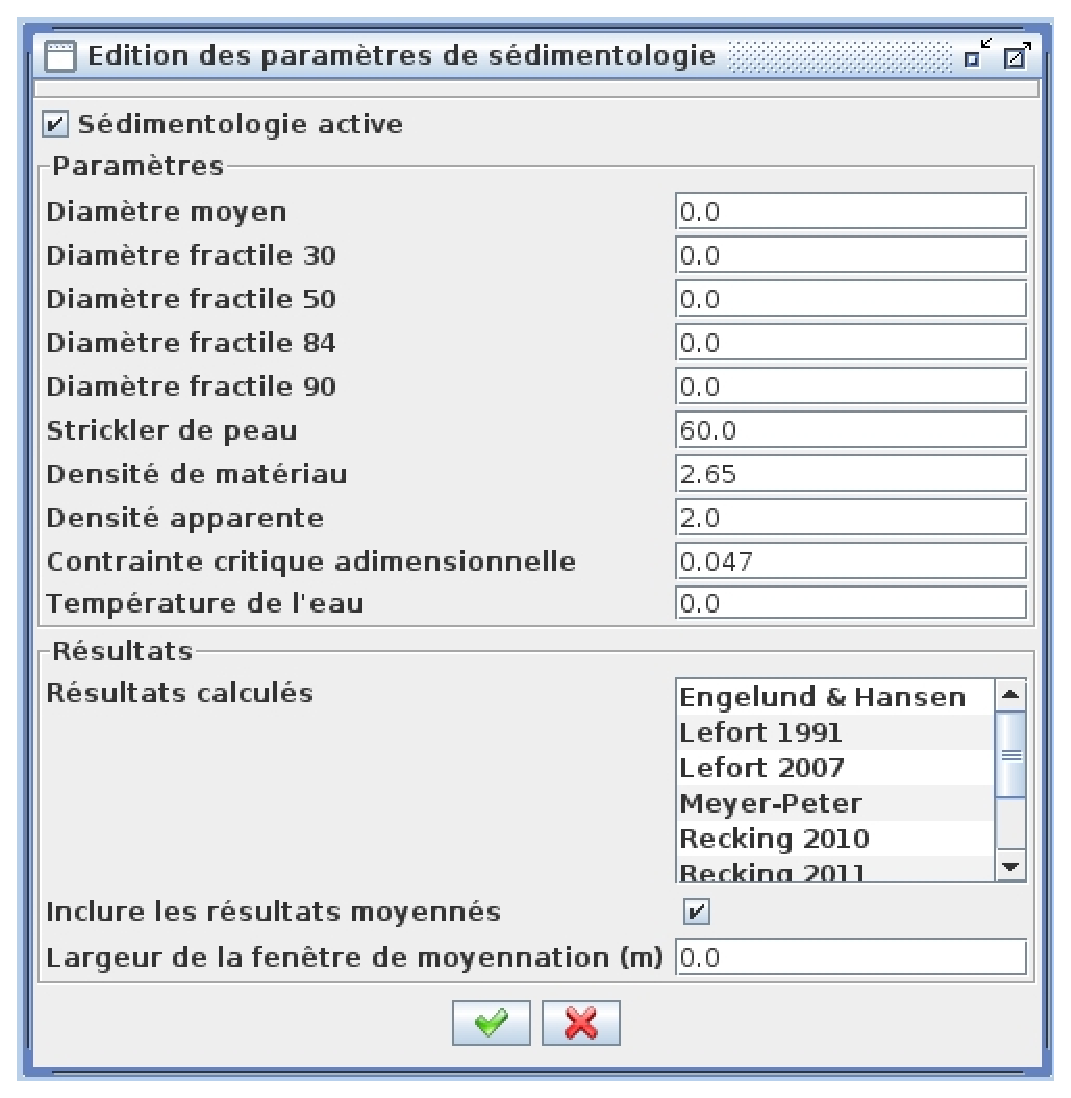
\includegraphics[scale=0.35]{mascapa}
  \caption{\label{fig}
  		   \textit{Edition des param\`etres de s\'edimentologie du module Fudaa-Mascapa.}}
 \end{center}
\end{figure}

\noindent
En les activant, l'utilisateur peut d\'efinir, dans la premi\`ere section \emph{``Param\`etres''}, les valeurs sedimentologiques tels que le diam\`etre moyen, le diam\`etre fractile $D_{30}$, le Strickler de peau, la densit\'e de mat\'eriau, etc. Les valeurs indiqu\'ees sur les cases \`a c\^ot\'e de chaque param\`etre sont des valeurs par d\'efaut. Elle doivent donc \^etre modifi\'ees par l'utilisateur en fonction du cas d'\'etude. Par exemple, la valeur par d\'efaut de Strickler de peau est de 60 $m^{1/3}/s$; elle est calcul\'ee pour un diam\`etre de grain de 1 mm avec la formule de Strickler. \\

\noindent
Dans la deuxi\`eme entr\'ee \emph{``R\'esultats''}, l'utilisateur choisit la formule pour calculer le d\'ebit solide. Il existe neuf formules qui peuvent \^etre utilis\'ees pour le m\^eme calcul. \\

\noindent
Enfin, pour tenir compte du lissage des fonds et donc des fluctuations des capacit\'es de transport solide, le calcul peut \^etre fait sur une moyenne mobile de longueur fix\'ee. Il est alors n\'ecesaire d'activer la case \`a cocher \emph{``Inclure les r\'esultats moyenn\'es'' } en bas de l'interface, en precisant la largeur de moyennation. \\


%%%%%%%%%%%%%%%%%%%%%%%%%%%%%%%%%%%%%%%%%%%%%%%%%%%%%%%%%%%%%%%%%%%%%%%%%%%%%%%%%%%%%%
%%%%%%%%%%%%%%%%%%%%%%%%%%%%%%%%%%%%%% RÉFÉRENCE %%%%%%%%%%%%%%%%%%%%%%%%%%%%%%%%%%%%%
%%%%%%%%%%%%%%%%%%%%%%%%%%%%%%%%%%%%%%%%%%%%%%%%%%%%%%%%%%%%%%%%%%%%%%%%%%%%%%%%%%%%%%
\newpage
\addcontentsline{toc}{section}{R\'ef\'erences}
\begin{thebibliography}{1}

\bibitem{gou1} \textsc{Goutal}, N., \textsc{Zaoui}, F., \textsc{Besnard}, A. $2007$. \emph{Note de principe syst\`eme mascaret v7p0}. Technical Report EDF-R\&D $H-P73-2007-0515$

\bibitem{lef1} \textsc{Lefort}, P. $2007$. Une formule semi-empirique pour le calcul du transport solide des rivi\`eres et torrents, paper presented at \emph{Transport solides et gestion des s\'ediments en milieux naturels et urbains}, 28-29 novembre, Lyon, SHF pp. $143-149$

\bibitem{rec2} \textsc{Recking}, A. $2010$. \emph{Evaluation des formules de transport solide en rivi\`ere avec prise en compte de l'\'echelle temporelle}. Rapport PGRN p. $30$

\bibitem{rec1} \textsc{Recking}, A., \textsc{Richard}, D., \textsc{Degoutte}, G. $2013$. \emph{Torrents et rivi\`eres de montagne dynamique et am\'enagement}. \'Editions Quae, France

\bibitem{rec3} \textsc{Recking}, A. $2012$. \emph{Cours d'hydraulique et de transport solide}. Master II, Paris 6

\bibitem{sma1} \textsc{Smart}, G.M., \textsc{J\"aggi}, M.N. $1983$. \emph{Sedimenttransport in steilen Gerinnen}. Versuchsanstalt f\"ur Wasserbau, Hydrologie und Glaziologie an der ETH Zurich p. $91$

\bibitem{van1} \textsc{Van Rijn}, L.C. $1993$. \emph{Principles of sediment transport in rivers, estuaries and coastal seas}. Aqua Publications, Amsterdam

\end{thebibliography}

%%%%%%%%%%%%%%%%%%%%%%%%%%%%%%%%%%%%%%%%%%%%%%%%%%%%%%%%%%%%%%%%%%%%%%%%%%%%%%%%%%%%%%
%%%%%%%%%%%%%%%%%%%%%%%%%%%%%%%%%%% FIN DU DOCUMENT %%%%%%%%%%%%%%%%%%%%%%%%%%%%%%%%%%
%%%%%%%%%%%%%%%%%%%%%%%%%%%%%%%%%%%%%%%%%%%%%%%%%%%%%%%%%%%%%%%%%%%%%%%%%%%%%%%%%%%%%%

\end{document}